\documentclass{beamer}
\usepackage[latin1]{inputenc}
%\usetheme[noshadow,nonav,nologo]{NYU}
\usetheme[numbers]{NYU}
\usepackage{amsmath}
\usepackage{amsfonts}
\usepackage{amssymb}

\title{Unsupervised Training using a Temporal Auto-Encoder Framework}
\date{April 30, 2014} 
\author{Ross Goroshin \hspace{0.20cm} Joan Bruna \hspace{0.20cm} Arthur Szlam \hspace{0.20cm} Yann LeCun}


\begin{document}

\begin{frame}
\titlepage
\end{frame}

\begin{frame}
\frametitle{Unsupervised Training using Video Data}  
\begin{center}
\begin{itemize} 
\item How can we train on the massive amounts of unlabeled video data available? 
\item Video is temporally coherent, thus it is reasonable to assume that neighboring frames are semantically similar
\item Use temporal coherence to develop new unsupervised learning objectives and train architectures (CNNs) that are able to satisfy them  
\item Video data can be considered as a form of 'correct' data augmentation, i.e. the variations observed are the variations on which to learn invariance/equivariance 
\end{itemize} 
\end{center}
\end{frame}

\begin{frame}
\frametitle{Slowness}  
\begin{center}
\begin{itemize} 
\item Extract features from individual frames that vary slowly with time, i.e. if $z_i = G_w(x_i)$ then $min~\|z_{i+1} - z_i\|_p$ 
\item Slow feature analysis: 
\begin{eqnarray} 
\nonumber 
&\text{Let }y_j(t):=g_j(x(t))&\\
\nonumber 
&min~\Delta(y_j):= \left <\dot y^2 \right >_t& \\
\nonumber
&s.t.~ \left <y_j \right >_t = 1 ~and~ \forall i<j: \left<y_i,y_j\right >_t = 0&
\end{eqnarray}
\item DrLIM: 
\begin{eqnarray} 
\nonumber
\text{Let } D_w(X_1, X_2) = \|G_w(X_{i+1})-G_w(X_i)\|_2 \\
\nonumber 
L = (1-Y)\frac{1}{2}D_W^2 + Y \frac{1}{2}(max(0,m-D_W))^2
\end{eqnarray} 
\end{itemize}
\end{center}
\end{frame}

\begin{frame} 
\frametitle{Slowness as Metric-Learning} 
\begin{center}
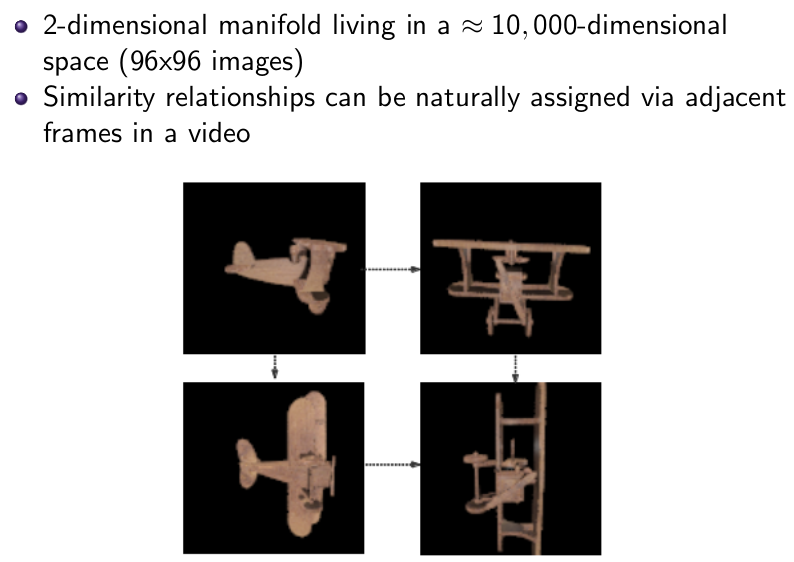
\includegraphics[scale=0.2]{./figures/drlim_data.png}
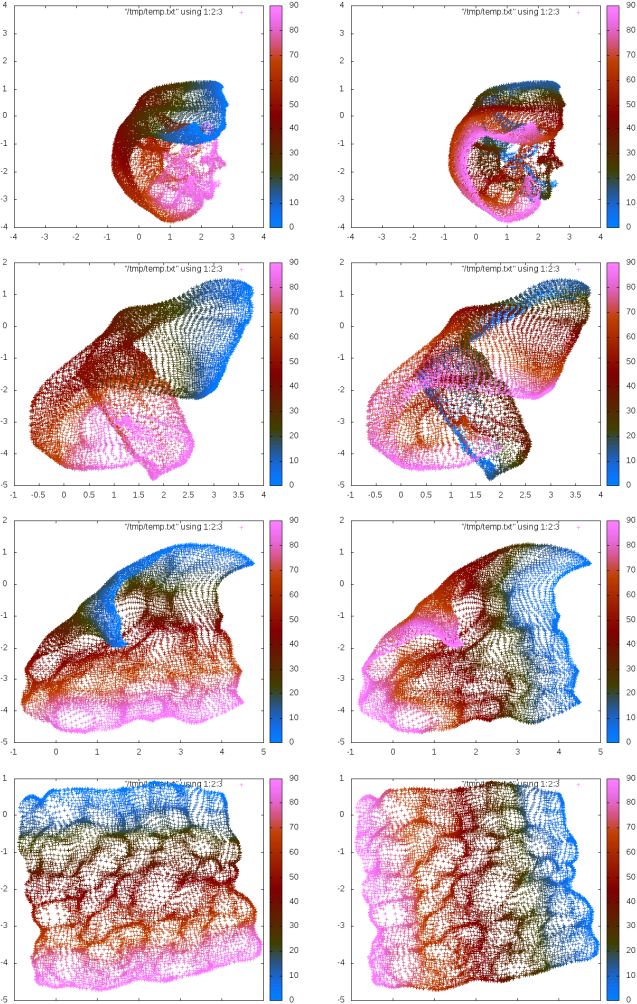
\includegraphics[scale=0.2]{./figures/drlim.png}
\end{center}
\end{frame} 

\begin{frame} 
\frametitle{Fully Connected Slow-Feature Auto-Encoders} 
Replacing the contrastive term in DrLIM with reconstruction lead to the slow-feature auto-encoder: 
\center
$L_{sample} = \sum_{i=1} ^2 \frac{1}{2}\|x_i - W_d~z_i\|^2 +\alpha|z_2 - z_1|$ \\ \vspace{0.5cm} 
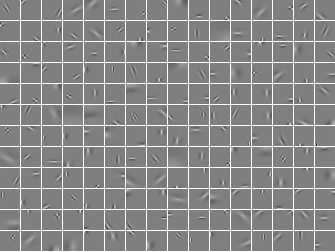
\includegraphics[scale=0.4]{./figures/SF.png} \hspace{0.5cm} 
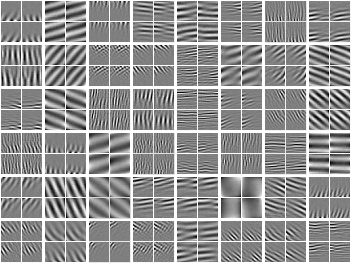
\includegraphics[scale=0.385]{./figures/fourier.png}\\
\hspace{1.5cm} No Pooling \hspace{3.5cm} $L_2$-Pooling
\end{frame} 

\begin{frame}
\frametitle{Fully Connected Slow-Feature Auto-Encoders} 
Introducing $L_1$ induces selective (localized, independent) features \\ \vspace{0.2cm} 
\small
$L_{sample} = \sum_{i=1} ^2 \frac{1}{2}\|x_i - W_d~z_i\|^2 +\alpha|\sqrt{\sum_N (z_2)^2} - \sqrt{\sum_N (z_1)^2}| + \beta(|z_1|+|z_2|)$\\
\begin{figure}
\center 
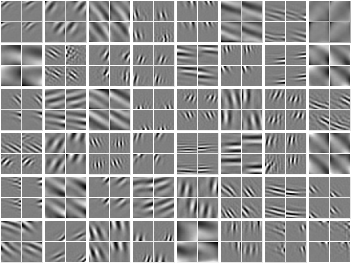
\includegraphics[scale=0.4]{./figures/L1_pool_SF.png} \hspace{0.5cm} 
\end{figure} 
\end{frame} 

\begin{frame} 
\frametitle{Decoding} 
\begin{figure} 
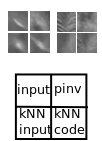
\includegraphics[scale=1]{./figures/example.png}
\end{figure} 
\end{frame} 

\begin{frame} 
\frametitle{YouTube Dataset} 
\begin{figure} 
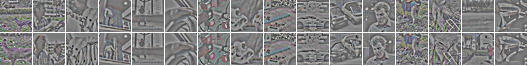
\includegraphics[scale=0.6]{./figures/sample.png}
\end{figure} 
\end{frame} 

\begin{frame}
\frametitle{YouTube Features} 
\begin{center} 
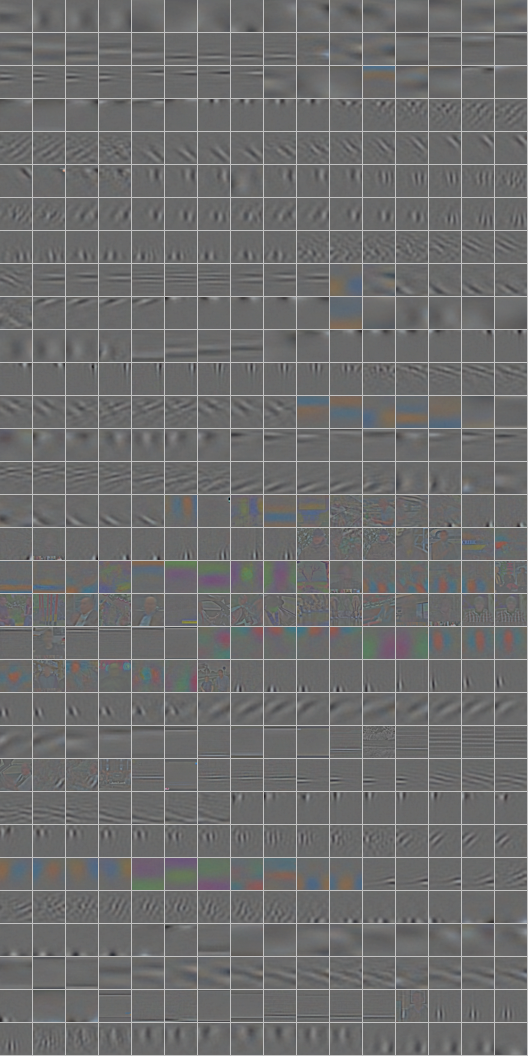
\includegraphics[scale=0.2]{./figures/sf_yt.png} \hspace{0.5cm} 
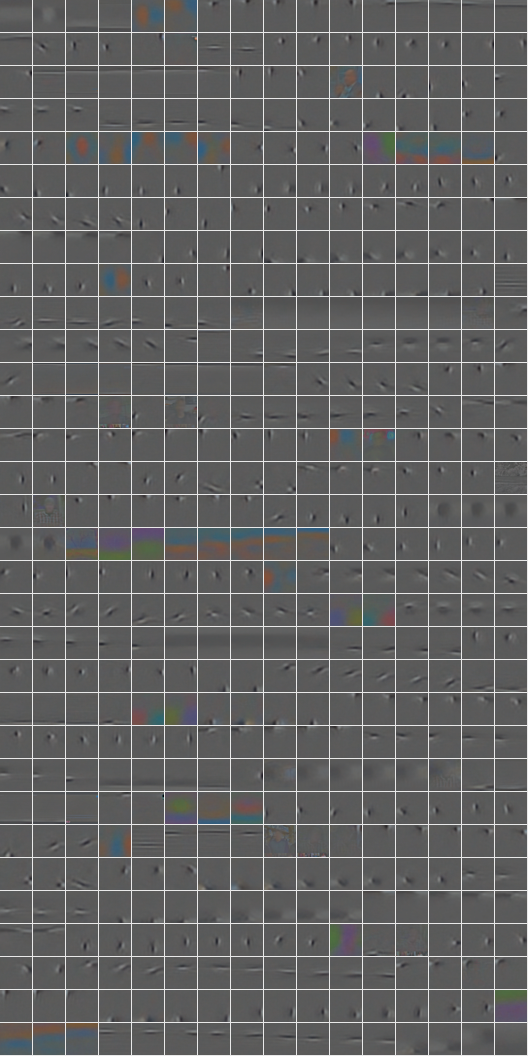
\includegraphics[scale=0.2]{./figures/gsc_yt.png} \hspace{0.5cm} 
\end{center} 
\end{frame} 

\begin{frame}
\frametitle{(Horrible) CIFAR-10 Performance}
\begin{itemize} 
\item Pre-training helps, but fully connected features can't compete with convolutional networks 
\end{itemize} 
\begin{centering} 
\begin{figure} 
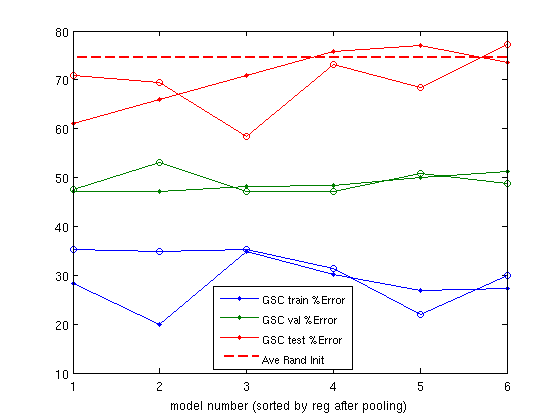
\includegraphics[scale=0.4]{./figures/class_graph.png} \hspace{0.5cm} 
\end{figure} 
\end{centering} 
\end{frame} 

\begin{frame}
\frametitle{Convolutional Feature Learning}  
\begin{itemize}
\item Convolutional dictionaries are massively over-complete, which makes sparse inference potentially more difficult
\item In the convolutional setting it may be necessary to have more sophisticated encoder (inference) to infer sparse codes 
\end{itemize} 
\begin{figure} 
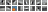
\includegraphics[scale=2]{./figures/dec_SC.png}
\caption{1. Sparse Coding using FISTA Inference}
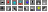
\includegraphics[scale=2]{./figures/LISTA1_dec.png}
\caption{2. Sparse Auto-Encoder using LISTA Encoder}
\end{figure} 
\end{frame} 

\begin{frame}
\frametitle{Convolutional LISTA}  
\begin{itemize}
\item Proposed Concern: weak encoder inference may prevent learning sparse features 
\item Proposed Solution: use a more powerful network specifically designed to perform sparse as the encoder  
\end{itemize} 
\begin{figure} 
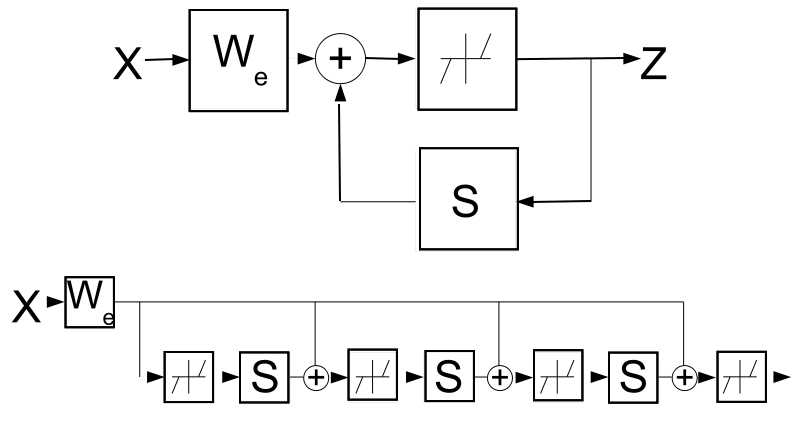
\includegraphics[scale=0.20]{./figures/LISTA.png}
\end{figure} 
\end{frame} 

\begin{frame} 
\frametitle{Code Prediction Performance}  
\begin{figure} 
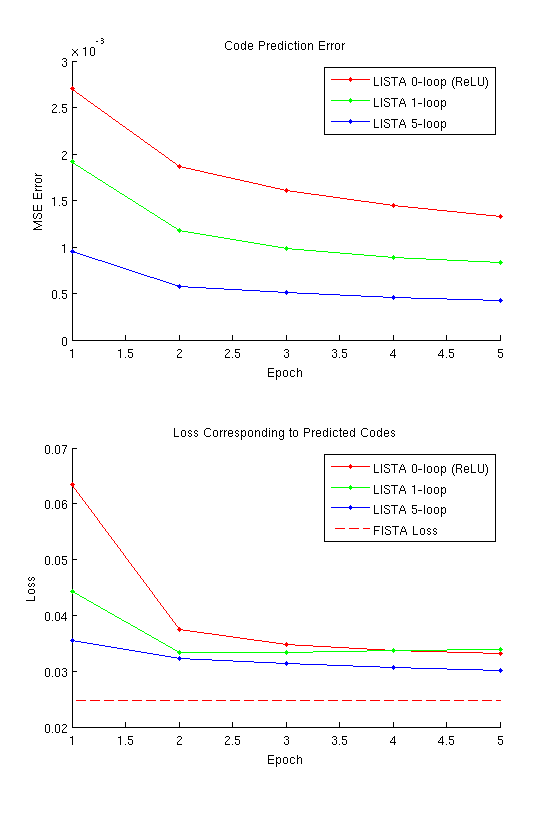
\includegraphics[scale=0.35]{./figures/code_pred.png}
\end{figure} 
\end{frame} 

\begin{frame} 
\frametitle{Inference Performance}  
\begin{figure} 
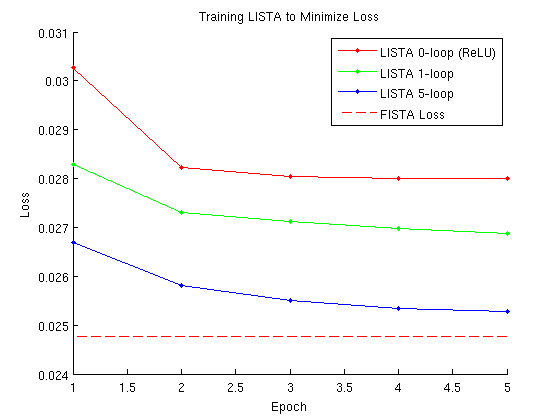
\includegraphics[scale=0.4]{./figures/LISTA_loss_min.png}
\end{figure} 
\small{However, in \emph{my} experiments I did not find that adding more than one-loop helps minimize the loss in dictionary learning} 
\end{frame} 

\begin{frame} 
\frametitle{Training a Single Stage CNN}
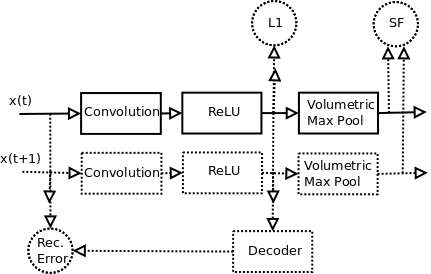
\includegraphics[scale=0.25]{./figures/standard_model.png}
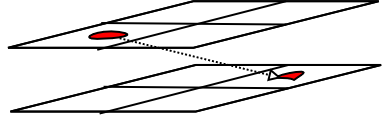
\includegraphics[scale=0.25]{./figures/volPool.png}\\
\begin{figure} 
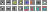
\includegraphics[scale=2]{./figures/dec16.png} \hspace{1cm} 
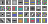
\includegraphics[scale=2]{./figures/dec32.png}
\caption{16 and 32 filter convolutional dictionary learned with volumetric max pooling in space (4x4) and features (2) }
\end{figure} 
\end{frame} 


\begin{frame}
\centerline{
\huge
\emph{Thank You}} 
\vspace{10 mm} 
\centerline{
\huge
\emph{THE END}} 

\end{frame}

\end{document}


